\section{Berbagai macam Jenis Sensor}
\section{Pengertian Sensor Suara}
Sensor suara merupakan sensor yang mensensing besaran suara untuk diubah menjadi besaran listrik. Sensor ini bekerja berdasarkan besar kecilnya kekuatan gelombang suara yang diterima. Dimana gelombang suara tersebut mengenai membran sensor, yang menyebabkan bergeraknya membran sensor yang memiliki kumparan kecil sehingga menghasilkan besaran listrik. Kecepatan bergeraknya kumparan kecil tersebut menentukan kuat lemahnya gelombang listrik yang akan dihasilkan. Salah satu contoh komponen yang termasuk dalam sensor ini adalah condeser microphone atau mic. Bentuk fisik dari condeser mic yaitu berbentuk bulat dan memiliki kaki dua seperti contoh pada gambar \ref{fig:sscondesermic}.
\begin{figure}[!htbp]
  \centering
  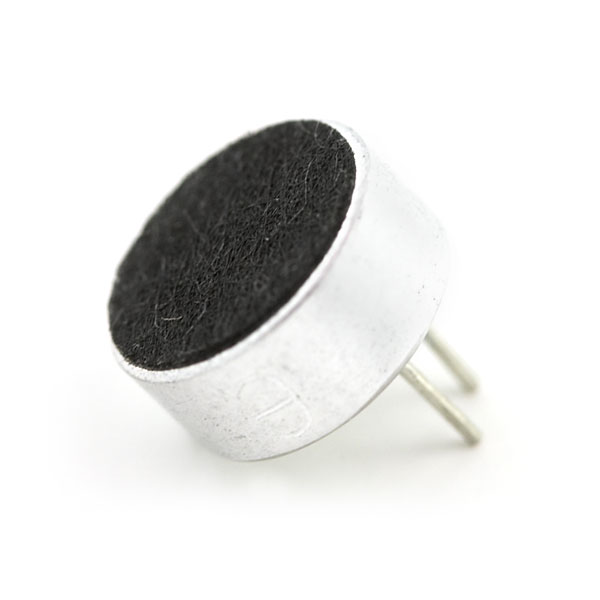
\includegraphics[width=.75\textwidth]{figures/Arduino/sscondesermic.jpg}
  \caption{Ini adalah Condeser Microphone}\label{fig:sscondesermic}
\end{figure}

\subsection{Prinsip Kerja Condeser Microphone}
Condenser mic biasanya bekerja berdasarkan susunan backplate atau diafragma yang harus terhubung dengan listrik dan membentuk kapasitor sound - sensitive. Gelombang suara yang tercipta akan masuk ke microphone dan akan menggetarkan komponen diafragma ini. Letak dari diafragma ditempatkan di depan sebuah backplate. Susunan dari elemen - elemen tersebut akan membentuk sebuah kapasitor yang sering disebut juga sebagai kondenser. Kapasitor memiliki kemampuan untuk menyimpan muatan maupun tegangan. Ketika elemen tersebut terisi dengan muatan, medan listrik akan terbentuk di antara diafragma dan backplate, yang dimana besarnya itu proporsional terhadap ruang yang terbentuk diantaranya. Macam - macam lebar dari jarak antara backplate dengan diafragma yang terjadi disebabkan karena adanya pergerakan oleh diafragma relatif terhadap backplate yang dikarenakan adanya tekanan suara yang mengenai diafragma. Hal ini akan menghasilkan sinyal elektrik dari gelombang suara yang masuk ke condenser microphone seperti contoh pada gambar \ref{fig:sscondesermicscheme}.
\begin{figure}[!htbp]
  \centering
  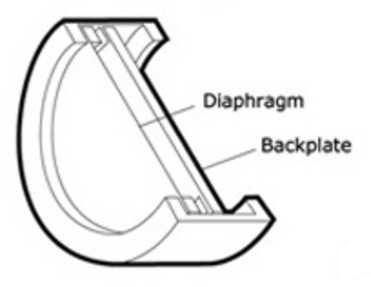
\includegraphics[width=.75\textwidth]{figures/Arduino/sscondesermicscheme.jpg}
  \caption{Ini adalah Skema dari Condeser Microphone}\label{fig:sscondesermicscheme}
\end{figure}

\subsection{Karakteristik dari Condeser Microphone}

Karakteristik dari Conseder Microphone adalah sebagai berikut :

\begin{enumerate}
  \item Susunannya lebih kompleks dibanding dengan jenis microphone lainnya seperti dibanding dengan dynamic Microphone.
  \item Pada frekuensi tinggi, akan menghasilkan suara yang lebih halus dan natural, serta sensitivitas yang lebih tinggi.
  \item Mudah akan mencapai respon frekuensi flat dan memiliki range frekuensi yang lebih luas.
  \item Ukurannya lebih kecil dibanding dengan jenis tipe mikrophone lainnya.
\end{enumerate}

Pada pasaran sudah dijual sensor suara menggunakan condeser mic ini dalam bentuk modul, sehingga mudah dan praktis dalam penggunaannya.

\begin{figure}[!htbp]
  \centering
  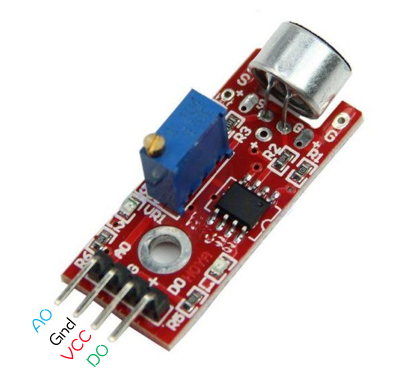
\includegraphics[width=.75\textwidth]{figures/Arduino/sssensorsuara.png}
  \caption{Ini adalah Skema dari Condeser Microphone}\label{fig:sssensorsuara}
\end{figure}	

Spesifikasi dari modul sensor suara seperti contoh pada gambar \ref{fig:sssensorsuara} adalah sebagai berikut :

\begin{enumerate}
  \item Sensitivitas dapat diatur (pengaturan manual pada potensiometer).
  \item Condeser yang digunakan memiliki sensitivitas yang tinggi.
  \item Tegangan kerja antara 3.3V – 5V.
  \item Terdapat 2 pin keluaran yaitu tegangan analog dan digital output.
  \item Sudah terdapat lubang baut untuk instalasi.
  \item Sudah terdapat indikator led.
\end{enumerate} 